\documentclass[12pt]{book}
\usepackage{booktabs}
\usepackage{tcolorbox}
\usepackage[T1]{fontenc}
\usepackage{wrapfig}
\usepackage[polish]{babel}
\usepackage[utf8]{inputenc}
\usepackage{lmodern}
\usepackage{pifont}
\usepackage{blkarray, bigstrut}
\usepackage{amsmath}
\usepackage{kbordermatrix}
\usepackage{cases}
\usepackage[T1]{fontenc}
\usepackage{amsthm}
\selectlanguage{polish}
\usepackage{amsmath}
\usepackage{graphicx}
\usepackage{float}
\usepackage[margin=2.5cm]{geometry}
\newcommand{\R}{\mathbb{R}}
\newcommand\addtag{\refstepcounter{equation}
\tag{\theequation}}
\begin{document}
\title{Optymalizacja  systemu sygnalizacji świetlnej w 
oparciu o przepływowy model ruchu pojazdów.}
\author{Michał Lis}
\date{\today}
\maketitle
\tableofcontents
\chapter{Wprowadzenie}
\chapter{Cel pracy}
\chapter{Zakres pracy}
   
   
\chapter{Siatka czasowa i przestrzenna}
Dyskretny charakter modelu przedstawianego w pracy obliguje do określenia siatki czasowej i przestrzennej. Dla par czasu i miejsc należących do tych dwóch siatek będą określane zmienne stanowe. \\ \\ \textbf{Siatka czasowa} jest zdefiniowana jako skończony ciąg liczb naturalnych:
\[(0,1,...,K). \addtag \]
Niech będzie ustalona droga $e$, która jest odcinkiem $[0,L_e]$. Droga zostaje podzielona na $L+1$ odcinków o równej długości $\Delta x=\frac{L_e}{L+1}$. \textbf{Siatka przestrzenna} drogi to ciąg odcinków:
\[(b_l)_{l=0}^{L}=[l\Delta x,(l+1)\Delta x]\]
\begin{figure}[H]
  \centering
    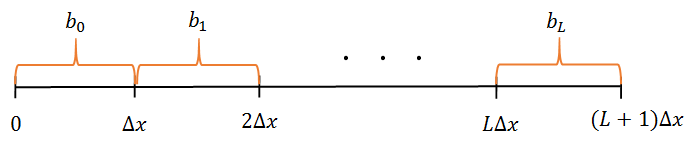
\includegraphics[width=14cm]{siatka_przestrzenna}
 \caption{Siatka przestrzenna}
 \label{fig:siatka_przestrzenna}
\end{figure}


\chapter{Makroskopowy model ruchu}
\section{Klasyfikacja modeli ruchu drogowego}
Modele ruchu drogowego mają na celu ukazanie rzeczywistego przepływu pojazdów w sposób czysto matematyczny. Ważnym kryterium doboru modelu jest przystępność jego implementacji informatycznej. Powszechnie klasyfikuje się 3 podejścia modelowe dla omawianego problemu \cite{CompareModels} - makroskopowy, mezoskopowy oraz mikroskopowy. Czasem \cite{multilevel} wyróżnia się także czwarte podejście - submikroskopowe. Jest to podział ze względu na poziom modelu. Najniższy poziom i najbardziej dokładny model gwarantuje podejście mikroskopowe. Rozważa ono pojazdy indywidualnie w czasoprzestrzeni. Przyspieszenie pojazdu jest wyliczane na podstawie dynamiki(prędkości, przyspieszenia) i pozycji pojazdu bezpośrednio przed nim. Model mezoskopowy zapewnia indywidualne rozróżnienie pojazdów, jednak ich zachowanie jest wyliczane na danych zagregowanych \cite{mesoscopic}. Przykładowo pojazdy są zgrupowane w grupę podróżującą z pewnego punktu startowego do celu. Inne modele \cite{mesoscopic2} mezoskopowe wyliczają dynamikę ruchu na podstawie aktualnego zatłoczenia drogi. Poziom mezoskopowy jest obliczeniowo bardziej opłacalny od mikroskopowego.
Wiele symulatorów stosujących model mezoskopowy oferuje symulację w czasie rzeczywistym dla sieci dróg całego miasta\cite{vu2017high}. Ideą modelu makroskopowego jest traktowanie ruchu ulicznego identycznie jak ruchu cieczy lub gazów. Po raz pierwszy w roku 1956 M. J. Lighthill i G. B. Whitham \cite{lwr} przedstawili pomysł przyrównania ruchu ulicznego na zatłoczonych drogach do przepływu wody w rzekach. Z tego powodu nie rozróżniamy w nim indywidualnie pojazdów, ani też nawet grupowo. Rozważamy natomiast gęstość ruchu w danym punkcie na drodze i czasie - czyli ilość pojazdów na danym odcinku drogi. Sposób w jaki poruszają się pojazdy jest wyliczany jedynie na podstawie gęstości ruchu. Jest to najmniej kosztowny obliczeniowo model. Właśnie w modelu makroskopowym zostało stworzone środowisko symulacyjne. Szczegóły modelu są przedstawione w następnym podrozdziale.

\section{Wstęp}
Istotą makroskopowego modelu ruchu jest pojęcie gęstości ruchu. Jest to zmienna stanowa określona dla każdego punktu drogi w czasie. Formalnie gęstość można rozumieć jako czynnik definiujący dynamikę ruchu. Im większa gęstość tym mniejsza prędkość ruchu. W niektórych artykułach gęstość ruchu \cite{helbing2001master} jest przedstawiona jako iloraz ilości pojazdów znajdujących się na pewnym odcinku i długości tego odcinka drogi. Nie są to jednak czysto matematyczne formalne definicje. W makroskopowym modelu nie rozróżniamy pojedynczych pojazdów, ani nawet grup, więc taka definicja gęstości ruchu może być odebrana jako nieścisła z ideą modelu. 
\section{Rozwój gęstości ruchu na drodze}
Makroskopowy model ruchu jest oparty o równanie różniczkowe (\ref{eq:main_diff_eq}) wraz z warunkiem początkowym (\ref{eq:p_init_eq}). Model makroskopowy traktuje ruch uliczny na drogach podobnie do przepływu wody w rzece[ref]. Gęstość ruchu można utożsamiać z polem powierzchni przekroju poprzecznego rzeki, co dla ustalonej szerokości rzeki - upraszcza się do wysokości wody w rzece. Istotną uwagą w tym miejscu jest zaznaczenie, iż rzeka zazwyczaj posiada pewien spadek, który zapewnia ruch cieczy ze źródła do ujścia. Ruch makroskopowy zdefiniowany przez równanie (\ref{eq:main_diff_eq}) z kolei odnosi się do rzeki która jest na całym swoim odcinku pozioma. W takim przypadku de facto nie ma zdefiniowanego zwrotu ruchu. \\Dla ustalonej drogi $e$ zmianę gęstości ruchu definiuje następujący układ równań:\\
\begin{numcases}{}
   p(x,0)=p_{0}(x) \label{eq:p_init_eq}
   \\
   \frac{\partial p(x,t)}{\partial t}+\frac{\partial f(p(x,t))}{\partial x}=0 \label{eq:main_diff_eq}
\end{numcases}
Gdzie $p(x,t)$ to gęstość ruchu w punkcie $x$ i czasie $t$. Wartość funkcji gęstości należy do przedziału $[0,p^{max}]$.\\
Równanie (\ref{eq:p_init_eq}) zakłada istnienie pewnej z góry nałożonej początkowej gęstości drogi $p_0(x)$.
Równianie (\ref{eq:main_diff_eq}) określa
wedle założeń modelu makroskopowego \cite{lwr} rozwój gęstości ruchu na drodze. Funkcja płynności ruchu $f$ powinna być wklęsła [ref]. W przedstawionym w tej pracy modelu funkcja ma następującą definicję:
\begin{numcases}{f(p)=}
   \lambda p & \text{dla } $p\in[0,p^{*}]$\\
   \lambda \cdot (2p^{*}-p) & \text{dla } $p\in(p^{*},p^{max}]$ 
\end{numcases}
Gdzie $\lambda$ jest stałym parametrem funkcji trójkątnej oraz $p^*=\frac{1}{2}p^{max}$.

\section{Dyskretyzacja makroskopowego modelu ruchu}
Niech będzie ustalona droga $e$ oraz jej siatka przestrzenna $b_l$. Celem jest przedstawienie wartości gęstości dla odcinków siatki przestrzennej w chwilach $k=0,1,...,K$.
Gęstość w odcinku $b_l$ i czasie $k$ jest zdefiniowana jako:
\[p_{l}^{k}=\int\limits_{{b_{l}}}{\frac{p(x,k)}{\Delta x}dx}. \addtag\]
Na podstawie (\ref{eq:main_diff_eq}) można wywnioskować, że:
\[\int\limits_{b_{l}} {p(x,k+1)- p(x,k)dx} +\int\limits_{k}^{k+1} f(b_{l+1},k)-f(b_{l},k))dk=0 \addtag \label{eq:calki-LWR} \]
Upraszczając otrzymujemy:
\[\Delta x(p_l^{k+1}-p_l^{k}) +\int\limits_{k}^{k+1} f(b_{l+1},k)-f(b_{l},k))dk=0=0 \addtag \]
Wartości gęstości zmieniają się w tylko w chwilach $k$. Wtedy wartości $f(b_{l+1},k)$ i $f(b_l,k)$ są stałe na całym przedziale całkowania $[k,k+1)$. Otrzymujemy równanie:
\[\Delta x(p_l^{k+1}-p_l^{k})  + (f(b_{l+1},k)-f(b_l,k))=0 \addtag \]
Rezultatem jest końcowy rekurencyjny wzór na gęstość ruchu:
\[p_l^{k+1}=p_l^{k}  -\frac{1}{\Delta x}  (f(b_{l+1},k)-f(b_l,k)) \addtag \]


\chapter{Model sieci dróg}
\section{Wstęp}
Ze względu na dużą złożoność końcowego modelu zostanie przedstawiony najpierw bardzo prosty, podstawowy model. W każdej kolejnej sekcji dodawane będą zmiany przybliżające do ostatecznej postaci. Jest to podejście pozwalające na proste przedstawienie modelu, który zawiera bardzo wiele aspektów m.in:
ujęcie sygnalizacji świetlnej, brak kolizyjnych manewrów, makroskopowy przepływ ruchu, przepływ ruchu na skrzyżowaniu, struktura sieci dróg. Zestawienie w jednej sekcji wszystkich tych kwestii byłoby bardzo przytłaczające.
\section{Symbole i notacja obliczeniowa}
Obliczenia w tym rozdziale będą wykonywane głównie na macierzach. Zazwyczaj macierze będą wyrazem ciągu, którego indeksem jest czas. Przykładowo $P(k)$ odnosi się do wartości w chwili $k$. Notacja $P(k,l)$ odnosi się do l-tej kolumny macierzy $P(k)$.\\
$\overrightarrow{P(k)}$ jest następującą operacją macierzową:
\begin{gather}
\overrightarrow{
  \begin{bmatrix}
   a_{11} & ... & a_{1m}\\
   ... & & ...\\
   a_{n1} & ... & a_{nm}\\
   \end{bmatrix}}
 =
  \begin{bmatrix}
   0 & a_{11} & ... & a_{1m-1}\\
   ... & ... & ... & ...\\
   0 & a_{n1} & ... & a_{nm-1}\\
   \end{bmatrix}
   \addtag
   \label{arrow_function}
\end{gather}
Jak łatwo zauważyć przesuwa ona wszystkie kolumny o jeden indeks w prawo. Pierwsza kolumna jest zerowa.
\section{Sieć dróg}
Sieć dróg przedstawia uporządkowana dwójka $G=(V,E)$, gdzie:
\begin{itemize}
\item $V$ to zbiór skrzyżowań
\item $E$ to zbiór dróg
\end{itemize}
\begin{minipage}{12cm}
\begin{figure}[H]
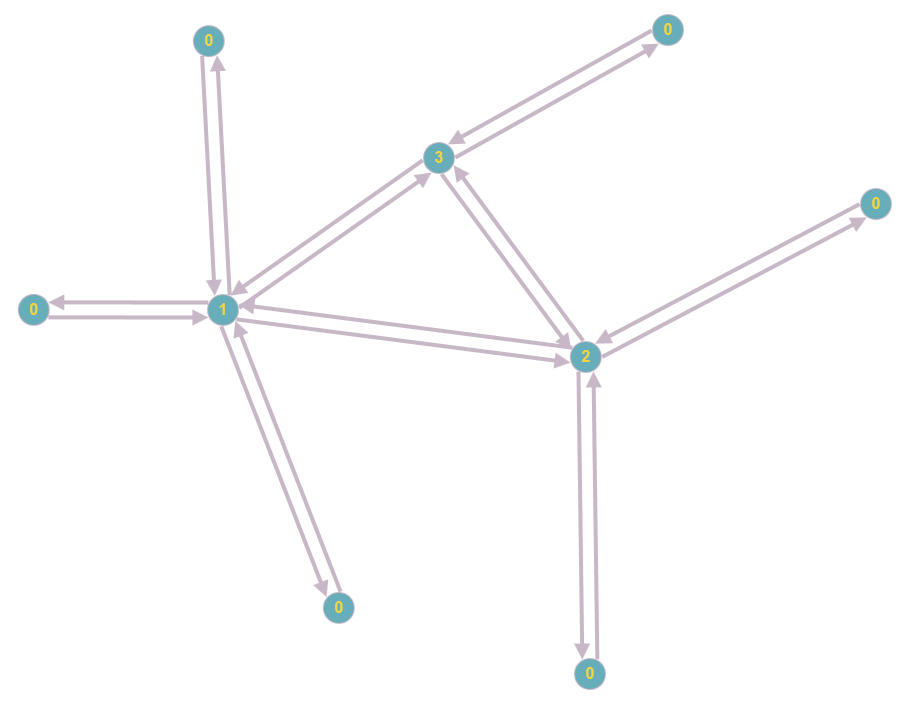
\includegraphics[width=12cm]{network}
\caption{\label{fig:network} Przykładowa sieć dróg}
\end{figure}
\end{minipage} \hfill
\begin{minipage}{5cm}
Skrzyżowania są oznaczone numerami: 1,2,3.
Punkty z numerem 0 są jedynie początkami i końcami dróg.
\end{minipage}
\newgeometry{left=0.8in,right=0.8in,top=1in,bottom=1in} \noindent
\section{Przykładowe skrzyżowanie}
Niech dane będzie skrzyżowanie dwóch dróg wlotowych $e_1,e_2$ i jednej wylotowej $e_3$. Każda z dróg jest jednakowej długości. Struktura skrzyżowania jest przedstawiona na rysunku \ref{fig:skrz_1}.
Macierz B jest \textbf{macierzą przejścia} skrzyżowania $v$. Wartości 1 oznaczają możliwy przejazd na skrzyżowaniu z drogi odpowiadającej indeksowi kolumny do drogi zadanej przez indeks wiersza.
\begin{equation*}
  B=
  \begin{blockarray}{*{3}{c} l}
    \begin{block}{*{3}{>{$\footnotesize}c<{$}} l}
     $e_1$ & $e_2$ & $e_3$\\
    \end{block}
    \begin{block}{[*{3}{c}]>{$\footnotesize}l<{$}}
       0 & 0 & 0 & $e_1$ \\
       0 & 0 & 0 & $e_2$ \\
       1 & 1 & 0 & $e_3$ \\
    \end{block}
  \end{blockarray} \addtag
\end{equation*}

\begin{figure}[H]
  \centering
    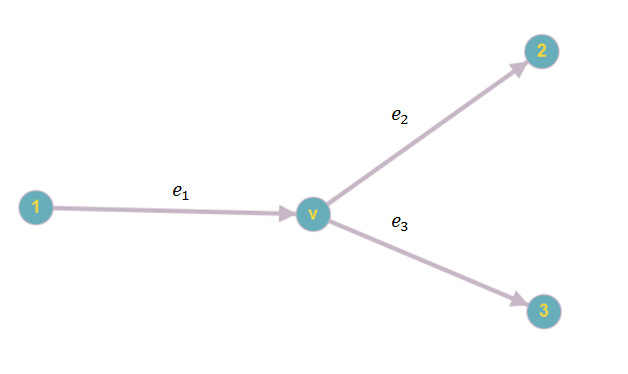
\includegraphics[width=14cm]{skrz_1}
 \caption{Skrzyzowanie 1}
 \label{fig:skrz_1}
\end{figure}


\section{Macierz stanowa sieci dróg}
Strukturą przedstawiającą stan sieci dróg jest \textbf{macierz stanowa} $P(k)$. Składuje ona zmienne stanowe w danym momencie $k$. Każdy wiersz macierzy odpowiada jednej drodze $e$. Indeks kolumny określa konkretny odcinek tej drogi. \\ \\ Wartość zmiennej stanowej początkowo jest ilością pojazdów na danym odcinku.
Jako przykład zostanie przedstawiona początkowa macierz stanowa skrzyżowania z rysunku \ref{fig:skrz_1}. Niech siatki przestrzenne dróg składają się z 4 odcinków. Początkowa macierz stanu $P(0)$ może być przedstawiona jako:
\begin{equation*}
  P(0)=
  \begin{blockarray}{*{4}{c} l}
    \begin{block}{*{4}{>{$\footnotesize}c<{$}} l}
      $b_0$ & $b_1$ & $b_2$ & $b_3$ \\
    \end{block}
    \begin{block}{[*{4}{c}]>{$\footnotesize}l<{$}}
       0 & 1 & 0 & 1 & $e_1$ \\
       0 & 0 & 0 & 1 & $e_2$ \\
       1 & 0 & 0 & 0 & $e_3$ \\
    \end{block}
  \end{blockarray} \addtag \label{skrz_1_x0}
\end{equation*}


Powyższa macierz przekazuje informację iż w chwili $0$ pojazdy są na następujących drogach:
\begin{itemize}
\item $e_1$ - na odcinkach $b_1,b_3$ 
\item $e_2$ - na odcinku $b_3$ 
\item $e_3$ - na odcinku $b_0$ 
\end{itemize}
\section{Model przepływu - przykład}
Początkowy model przepływu pojazdów zakłada, iż wszystkie pojazdy w chwili $k+1$ są o jeden odcinek dalej w swojej podróży niż w momencie $k$. Założone jest iż żadne nowe pojazdy nie pojawiają się w sieci dróg, a pojazdy będące w chwili $k$ w ostatnim odcinku drogi $e_3$ opuszczają układ. Wtedy kolejne macierze stanowe dla przykładu \ref{skrz_1_x0} są następujące:
\begin{equation*}
  P(1)=
  \begin{blockarray}{*{4}{c} l}
    \begin{block}{*{4}{>{$\footnotesize}c<{$}} l}
      $b_0$ & $b_1$  & $b_2$ & $b_3$ \\
    \end{block}
    \begin{block}{[*{4}{c}]>{$\footnotesize}l<{$}}
       0 & 0 & 1 & 0 & $e_1$ \\
       0 & 0 & 0 & 0 & $e_2$ \\
       2 & 1 & 0 & 0 & $e_3$ \\
    \end{block}
  \end{blockarray} \addtag
\end{equation*}

\begin{equation*}
  P(2)=
  \begin{blockarray}{*{4}{c} l}
    \begin{block}{*{4}{>{$\footnotesize}c<{$}} l}
      $b_0$ & $b_1$ & $b_2$ & $b_3$  \\
    \end{block}
    \begin{block}{[*{4}{c}]>{$\footnotesize}l<{$}}
       0 & 0 & 0 & 1 & $e_1$ \\
       0 & 0 & 0 & 0 & $e_2$ \\
       0 & 2 & 1 & 0 & $e_3$ \\
    \end{block}
  \end{blockarray} \addtag
\end{equation*}


\begin{equation*}
  P(3)=
  \begin{blockarray}{*{4}{c} l}
    \begin{block}{*{4}{>{$\footnotesize}c<{$}} l}
      $b_0$ & $b_1$ & $b_2$ & $b_3$ \\
    \end{block}
    \begin{block}{[*{4}{c}]>{$\footnotesize}l<{$}}
       0 & 0 & 0 & 0 & $e_1$ \\
       0 & 0 & 0 & 0 & $e_2$ \\
       1 & 0 & 2 & 1 & $e_3$ \\
    \end{block}
  \end{blockarray} \addtag
\end{equation*}

\begin{equation*}
  P(4)=
  \begin{blockarray}{*{4}{c} l}
    \begin{block}{*{4}{>{$\footnotesize}c<{$}} l}
     $b_0$ & $b_1$ & $b_2$ & $b_3$ \\
    \end{block}
    \begin{block}{[*{4}{c}]>{$\footnotesize}l<{$}}
       0 & 0 & 0 & 0 & $e_1$ \\
       0 & 0 & 0 & 0 & $e_2$ \\
       0 & 1 & 0 & 2 & $e_3$ \\
    \end{block}
  \end{blockarray} \addtag
\end{equation*}

\section{Model przepływu - ogólny wzór}
W poprzedniej sekcji został przedstawiony przykład wyliczenia macierzy stanowej dla kolejnych momentów w czasie. Następnym krokiem jest przedstawienie rozwiązania dla ogólnego przypadku. \\ 

\begin{tcolorbox}

Ogólny wzór przedstawiający rozwój macierzy stanowej to:
\[P(k+1)=\overrightarrow{P(k)} + S(k) \addtag \label{eq:P}\]
Macierz $S(k)$ nazywana będzie \textbf{macierzą źródła}. Dotyczy ona ruchu wpływającego do poszczególnych dróg w momencie $k+1$. Jest to macierz rzadka, istotna obliczeniowo jest jedynie pierwsza kolumna, a pozostałe wartości są zerowe by osiągnąć wymiar macierzy pozwalający na dodawanie z $\overrightarrow{P(k)}$. Pierwsza kolumna jest zdefiniowana w oparciu o ostatnią kolumnę macierzy $P(k)$ i jest równa:
\[S(k,0)=B\cdot P(k,l) \addtag \label{eq:S} \]
\end{tcolorbox} \noindent
Dla przykładu z poprzedniej sekcji, gdzie
\[P(0)= \begin{bmatrix} 0 & 1 & 0 & 1\\
       0 & 0 & 0 & 1 \\
       1 & 0 & 0 & 0 \end{bmatrix}\]
Dla kolejnego momentu $k=1$ korzystając ze wzoru (\ref{eq:P}):
\[P(1)=\overrightarrow{P(0)}+S(0) \addtag \label{eq:P_1} \]
Należy wyliczyć macierz źródła, jej pierwsza kolumna to:
\[S(0,0)=B\cdot P(0,l)=
  \begin{bmatrix}
   0 & 0 & 0\\
   0 & 0 & 0\\
   1 & 1 & 0\\
   \end{bmatrix}
   \cdot
   \begin{bmatrix}
   1\\
   1\\
   0\\
   \end{bmatrix}
   =
      \begin{bmatrix}
   0\\
   0\\
   2\\
   \end{bmatrix}
 \]
 Zatem 
 \[S(0)=\begin{bmatrix}
 0 & 0 & 0 & 0\\
 0 & 0 & 0 & 0\\
 2 & 0 & 0 & 0\\
 \end{bmatrix}\]
 Oczywiście
 \[ \overrightarrow{P(0)}=
\begin{bmatrix}
 0 & 0 & 1 & 0\\
 0 & 0 & 0 & 0\\
 0 & 1 & 0 & 0\\
 \end{bmatrix} 
 \]
  
Ostatecznie ze wzoru (\ref{eq:P_1}) wynika, że
 \[P(1)=\begin{bmatrix}
 0 & 0 & 1 & 0\\
 0 & 0 & 0 & 0\\
 0 & 1 & 0 & 0\\
 \end{bmatrix}+
 \begin{bmatrix}
 0 & 0 & 0 & 0\\
 0 & 0 & 0 & 0\\
 2 & 0 & 0 & 0\\
 \end{bmatrix}=
  \begin{bmatrix}
 0 & 0 & 1 & 0\\
 0 & 0 & 0 & 0\\
 2 & 1 & 0 & 0\\
 \end{bmatrix}
 \]
Warto zauważyć, że w chwili 0 na obydwu drogach wlotowych $e_1,e_2$ pojazdy znajdowały się na końcowym odcinku. Problemem okazuje się kolizyjność manewrów wjazdu na drogę $e_3$ z dróg odpowiednio $e_1$ i $e_2$. Początkowo ta kwestia została ona pominięta. Następna sekcja przedstawia rozwiązanie tego problemu.
\section{Model przepływu z sygnalizacją świetlną - przykład}
\begin{figure}[H]
  \centering
    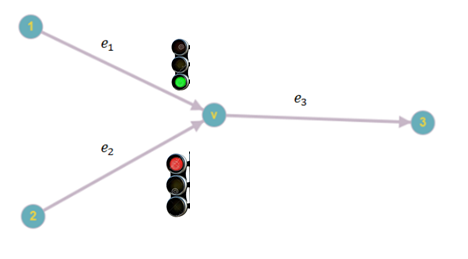
\includegraphics[width=14cm]{skrz_1_sygnalizacja}
 \caption{Skrzyzowanie 1 z sygnalizacją świetlną w chwili 0}
 \label{fig:skrz_1_sygnalizacja}
\end{figure}

Wprowadzona zostaje sygnalizacja świetlna dla dwóch dróg wlotowych $e_1$,$e_2$. Sygnalizacja świetlna będzie oparta o ciąg \textbf{macierzy sygnalizacji}. Określają one z której drogi pojazdy będą mogły wjechać na drogę $e_3$. Dla chwili 0 przyjęte jest, że zgodnie z rysunkiem \ref{fig:skrz_1_sygnalizacja} pojazdy na ostatnim odcinku drogi $e_2$ będą musiały poczekać. 
Przykładowa początkowa macierz to:
\begin{equation*}
  M(0)=
  \begin{blockarray}{*{3}{c} l}
    \begin{block}{*{3}{>{$\footnotesize}c<{$}} l}
     $e_1$ & $e_2$ & $e_3$\\
    \end{block}
    \begin{block}{[*{3}{c}]>{$\footnotesize}l<{$}}
       0 & 0 & 0 & $e_1$ \\
       0 & 0 & 0 & $e_2$ \\
       \textbf{1} & \textbf{0} & 0 & $e_3$ \\
    \end{block}
  \end{blockarray} \addtag
\end{equation*}

Przekazuje ona informację, że:
\begin{itemize}
\item Jest zielone światło na drodze $e_1$ w chwili 0 
\item Jest czerwone światło na drodze $e_2$ w chwili 0
%\item Pogrubione wartości odnoszą się do manewru posiadającego sygnalizację świetlna.
%\item Niepogrubione wartości równe 0 odnoszą się do sytuacji gdy nie istnieje pożądany manewr.
%\item Niepogrubione wartości równe 1 dotyczą dwóch tych samych dróg.
\end{itemize}

Poniższy przykład obrazuje rozwój macierzy stanowej dla skrzyżowania z sygnalizacją świetlną.
\begin{equation*}
  P(0)=
  \begin{blockarray}{*{4}{c} l}
    \begin{block}{*{4}{>{$\footnotesize}c<{$}} l}
      $b_0$ & $b_1$ & $b_2$ & $b_3$ \\
    \end{block}
    \begin{block}{[*{4}{c}]>{$\footnotesize}l<{$}}
       0 & 1 & 0 & 1 & $e_1$ \\
       0 & 1 & 0 & 1 & $e_2$ \\
       1 & 0 & 0 & 0 & $e_3$ \\
    \end{block}
  \end{blockarray} \addtag \label{skrz_1_zmiennaStanu_0_sygnalizacja}
\end{equation*}
Zgodnie z rysunkiem \ref{fig:skrz_1_sygnalizacja} czerwone światło na drodze $e_2$ powoduje, że pojazdy nie opuszczają ostatniego odcinka tej drogi. Z kolei pojazdy ostatniego odcinka drogi $e_1$ wjeżdżają na drogę $e_3$. Zatem: 
\begin{equation*}
  P(1)=
  \begin{blockarray}{*{4}{c} l}
    \begin{block}{*{4}{>{$\footnotesize}c<{$}} l}
      $b_0$ & $b_1$ & $b_2$ & $b_3$ \\
    \end{block}
    \begin{block}{[*{4}{c}]>{$\footnotesize}l<{$}}
       0 & 0 & 1 & 0 & $e_1$ \\
       0 & 0 & 1 & 1 & $e_2$ \\
       1 & 1 & 0 & 0 & $e_3$ \\
    \end{block}
  \end{blockarray} \addtag \label{skrz_1_zmiennaStanu_0_sygnalizacja}
\end{equation*}
Sygnalizacja świetlna nie zmienia się w chwili 1. Dochodzi do sytuacji gdy ruch kumuluje się na ostatnim odcinku drogi $e_2$.
\begin{equation*}
  P(2)=
  \begin{blockarray}{*{4}{c} l}
    \begin{block}{*{4}{>{$\footnotesize}c<{$}} l}
      $b_0$ & $b_1$ & $b_2$ & $b_3$ \\
    \end{block}
    \begin{block}{[*{4}{c}]>{$\footnotesize}l<{$}}
       0 & 0 & 0 & 1 & $e_1$ \\
       0 & 0 & 0 & 2 & $e_2$ \\
       0 & 1 & 1 & 0 & $e_3$ \\
    \end{block}
  \end{blockarray} \addtag \label{skrz_1_zmiennaStanu_0_sygnalizacja}
\end{equation*}
Niech w chwili 2 będzie zielone światło dla drogi $e_2$, czyli
\begin{equation*}
  M(2)=
  \begin{blockarray}{*{3}{c} l}
    \begin{block}{*{3}{>{$\footnotesize}c<{$}} l}
     $e_1$ & $e_2$ & $e_3$\\
    \end{block}
    \begin{block}{[*{3}{c}]>{$\footnotesize}l<{$}}
       0 & 0 & 0 & $e_1$ \\
       0 & 0 & 0 & $e_2$ \\
       \textbf{0} & \textbf{1} & 0 & $e_3$ \\
    \end{block}
  \end{blockarray} \addtag
\end{equation*}
Początkowo założone jest, że wszystkie pojazdy na ostatnim odcinku drogi przejeżdżają przez skrzyżowanie. Wtedy:
\begin{equation*}
  P(3)=
  \begin{blockarray}{*{4}{c} l}
    \begin{block}{*{4}{>{$\footnotesize}c<{$}} l}
      $b_0$ & $b_1$ & $b_2$ & $b_3$ \\
    \end{block}
    \begin{block}{[*{4}{c}]>{$\footnotesize}l<{$}}
       0 & 0 & 0 & 1 & $e_1$ \\
       0 & 0 & 0 & 0 & $e_2$ \\
       2 & 0 & 1 & 1 & $e_3$ \\
    \end{block}
  \end{blockarray} \addtag \label{skrz_1_zmiennaStanu_0_sygnalizacja}
\end{equation*}

\section{Model przepływu z sygnalizacją świetlną - ogólny wzór}

Następnym krokiem jest wyznaczenie ogólnego wzoru macierzy stanowej z uwzględnieniem sygnalizacji świetlnej. 
\begin{tcolorbox}
Macierz źródła z uwzględnieniem sygnalizacji świetlnej jest przedstawiona wzorem:
\[S(k,0)=M(k) \cdot P(k,l) \addtag \label{eq:S} \]
Oprócz pierwszej kolumny macierz $S$ dalej posiada wartości zerowe.\\
Wprowadzony zostanie ciąg $W(k)$ pomocniczych \textbf{macierzy oczekujących pojazdów}. Będą to macierze rzadkie z wartościami innymi niż 0 tylko w ostatniej kolumnie. Macierze te będą składowały informację o pojazdach oczekujących na zielone światło w swojej ostatniej kolumnie. Jest ona zdefiniowana jako:
\[W(k,l)=P(k,l)-S(k,0)\]

Wzór określający rozwój macierzy stanowej jest następujący:

\[P(k+1)=\overrightarrow{P(k)} + S(k) + W(k) \addtag \label{eq:P_sygnalizacja}\]
\end{tcolorbox}
\newpage 
Dla wcześniej przedstawionego przykładu w tabeli są wypisane obliczenia wedle wzoru (\ref{eq:P_sygnalizacja}).

\def \PZero { $\begin{bmatrix}
0 & 1 & 0 & \textbf{1}  \\
0 & 1 & 0 & 1  \\
1 & 0 & 0 & 0  
\end{bmatrix}$
}
\def \PmovedZero {
$\begin{bmatrix}
0 & 0 & 1 & 0  \\
0 & 0 & 1 & 0  \\
0 & 1 & 0 & 0  
\end{bmatrix}$
}
\def \SZero {
$\begin{bmatrix}
1 \\
0 \\
0   
\end{bmatrix}$

}
\def \WZero {
$\begin{bmatrix}
0  \\
1  \\
0  
\end{bmatrix}$
}
\def \MZero {$\begin{bmatrix}
  0 & 0 & 0 \\
       0 & 0 & 0\\
       1 & 0 & 0 \\
\end{bmatrix}$}


\def \PI {
$\begin{bmatrix}
0 & 0 & 1 & \textbf{0}  \\
0 & 0 & 1 & 1  \\
1 & 1 & 0 & 0  
\end{bmatrix}$
}
\def \PmovedI {
$\begin{bmatrix}
0 & 1 & 0 & 1  \\
0 & 0 & 0 & 1  \\
0 & 0 & 1 & 0  
\end{bmatrix}$
}
\def \SI {
$\begin{bmatrix}
0  \\
0  \\
0  
\end{bmatrix}$
}
\def \WI {$\begin{bmatrix}
0  \\
1  \\
0  
\end{bmatrix}$}
\def \MI {$\begin{bmatrix}
0 & 0 & 0  \\
0 & 0 & 0  \\
1 & 0 & 0  
\end{bmatrix}$}


\def \PII {$\begin{bmatrix}
0 & 1 & 0 & 1  \\
0 & 0 & 0 & \textbf{2}  \\
0 & 1 & 1 & 0  
\end{bmatrix}$}
\def \PmovedII {$\begin{bmatrix}
0 & 0 & 1 & 0  \\
0 & 0 & 0 & 0  \\
0 & 0 & 0 & 1  
\end{bmatrix}$}
\def \SII {
$\begin{bmatrix}
0  \\
2  \\
0  
\end{bmatrix}$}
\def \WII {$\begin{bmatrix}
1  \\
0  \\
0  
\end{bmatrix}$}
\def \MII {$\begin{bmatrix}
  0 & 0 & 0 \\
       0 & 0 & 0\\
       0 & 1 & 0 \\
\end{bmatrix}$}


\def \PIII {
$\begin{bmatrix}
  0 & 0 & 1 & 1 \\
  2 & 0 & 0 & 0 \\
  0 & 0 & 0 & 1 \\
\end{bmatrix}$
}
\def \PmovedIII {}
\def \SIII {}
\def \WIII {}
\def \MIII {}

\begin{table}[ht]
\caption{Rozwój macierzy stanowej na skrzyżowaniu 1 z sygnalizacją świetlną}
\centering
\begin{tabular}{|c|c|c|c|c|c|} \hline
k & M(k)& P(k) & $\overrightarrow{P(k)}$ & S(k,0) & W(k,l) \rule{0pt}{18pt} \\
\hline
0 & \MZero & \PZero & \PmovedZero & \SZero & \WZero \rule{0pt}{35pt} \\  
1 & \MI    &\PI    &\PmovedI   &\SI   &\WI   \rule{0pt}{35pt} \\
2 & \MII   &\PII   &\PmovedII  &\SII  &\WII  \rule{0pt}{35pt} \\
3 & \MIII  &\PIII  &\PmovedIII &\SIII &\WIII \rule{0pt}{35pt} \\
\hline
\end{tabular}
\label{Tab:Tcr}
\end{table}
\noindent
Pogrubione wartości odnoszą się do pojazdów, które przejeżdżają w momencie $k$ przez skrzyżowanie.





\bibliographystyle{IEEEtran}
\bibliography{refs}
\end{document}
